\documentclass[10pt,a4paper,usenames,dvipsnames]{beamer}
\usepackage[utf8]{inputenc}
\usepackage{lmodern}
\usepackage[T1]{fontenc}
\usepackage{xcolor,amsmath,tikz,graphicx,mathtools}
\usepackage{listings,algpseudocode,url}
\usepackage{slashed}

\usetheme{corporate}
\usefonttheme[onlymath]{serif}

\usetikzlibrary{calc,positioning}

\renewcommand{\rightarrow}{\text{\tikz[baseline=-0.25em]{%
\draw[opacity=0] (-0.1,0) -- (0.5,0);
\draw[->,>=stealth] (0,0) -- (0.4,0);
}}}

%\renewcommand{\leftrightarrow}{\text{\tikz[baseline=-0.25em]{%
%\draw[opacity=0] (-0.1,0) -- (0.5,0);
%\draw[->,>=stealth] (0,0) -- (0.4,0);
%}}}

\renewcommand{\hookrightarrow}{\text{\tikz[baseline=-0.25em]{%
\draw (0,0) arc (270:90:0.04);
\draw[->,>=stealth] (0,0) -- (0.4,0);
}}}

\title[Chiral Phase Transition]{The Chrial Phase Transition in QCD}
\subtitle{Mean-Field $\leftrightarrow$ Funtional Renormalisation Group}
\author[Glesaaen]{Aleksandra R. Glesaaen}
\institute[Goethe-Uni]{Goethe Universit\"{a}t Frankfurt am Main}
\date{3. February 2014}

\begin{document}

\begin{frame}[plain]
  \titlepage

  \begin{tikzpicture}[overlay, remember picture]
    \node[color=white, scale=0.8, anchor=west] at ([shift={(-3cm, -3cm)}] current page.center) {
        in collaboration with Prof. J.O. Andersen (NTNU)
      };
  \end{tikzpicture}
\end{frame}

\addtocounter{framenumber}{-1}

\begin{frame}
  \frametitle{Motivation}
  
  \begin{columns}[c]
    \column{.4\textwidth}
    \begin{itemize} \itemsep20pt
      \item<1-> Heavy Ion Collisions \\ (RHIC, LHC, FAIR)
      \item<2-> Dense-massive stars
      \item<3-> The $T$-$\mu$ phase diagram of QCD
    \end{itemize}
    \column{.6\textwidth}
    \only<1>{%
      \begin{tikzpicture}
        \node at (0,0) (alice) {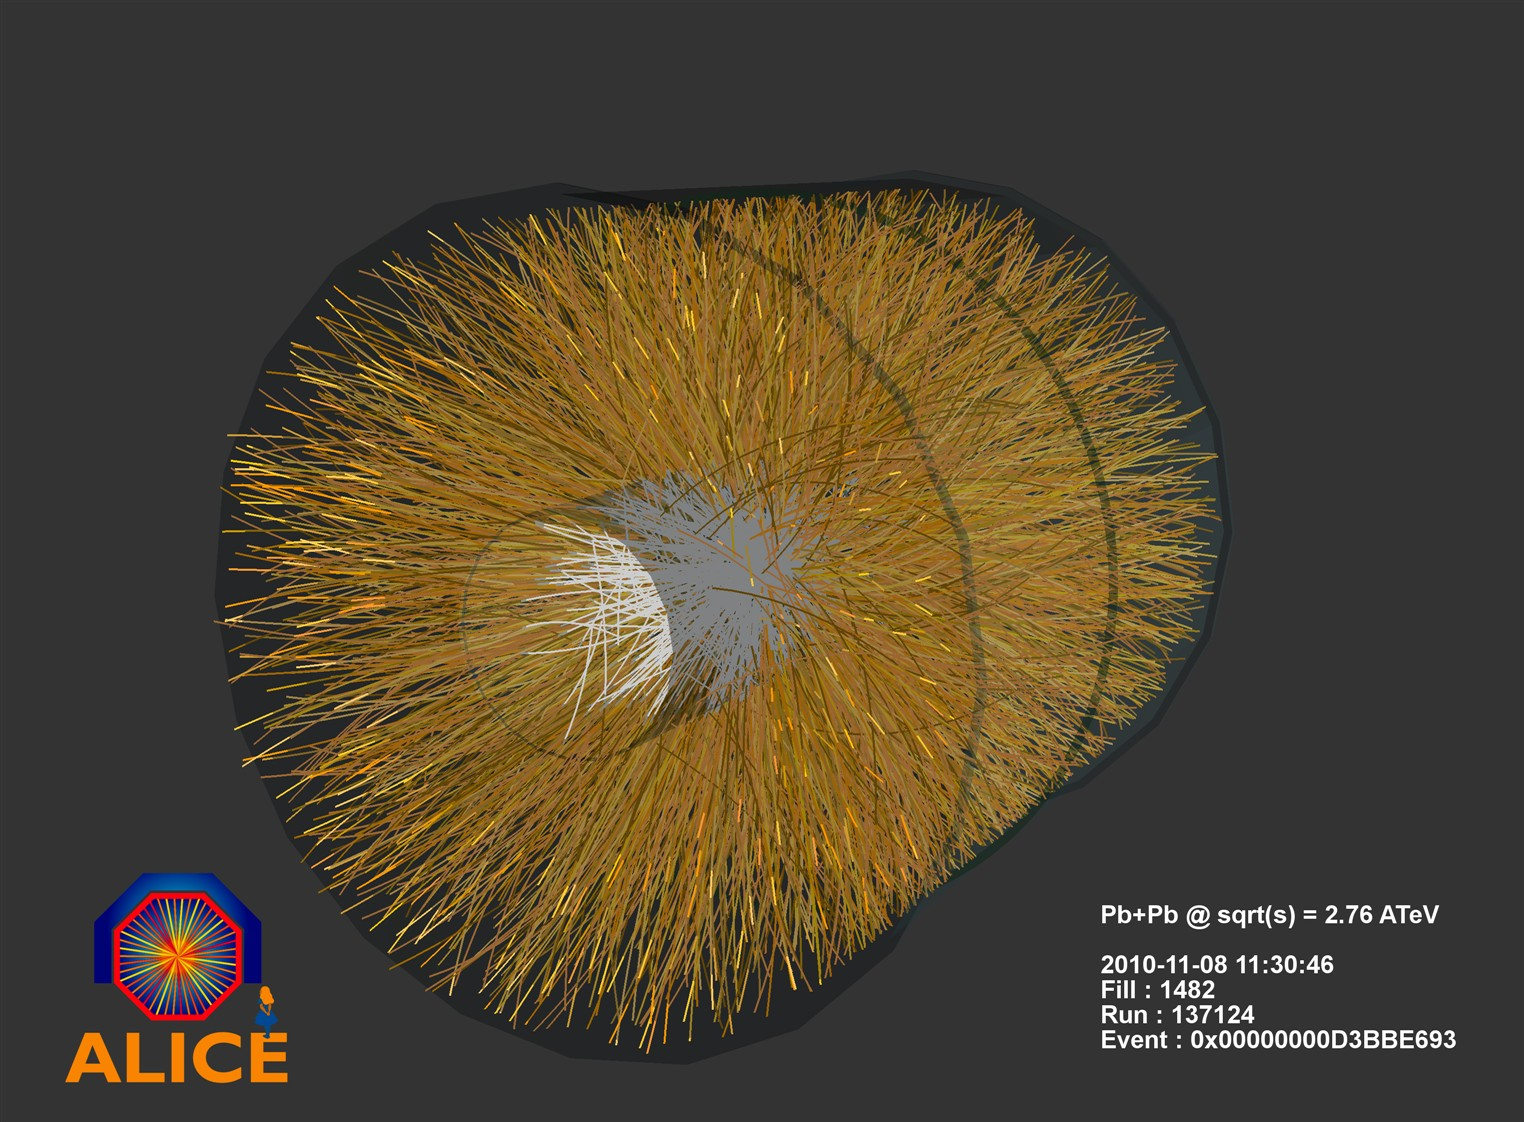
\includegraphics[width=.7\textwidth]{Pictures/alice.jpg}};
        \node at (alice.south){\tiny Picture taken from \url{cern.ch}};
      \end{tikzpicture}
    }
    \only<2>{%
      \begin{tikzpicture}
        \node at (0,0) (alice) {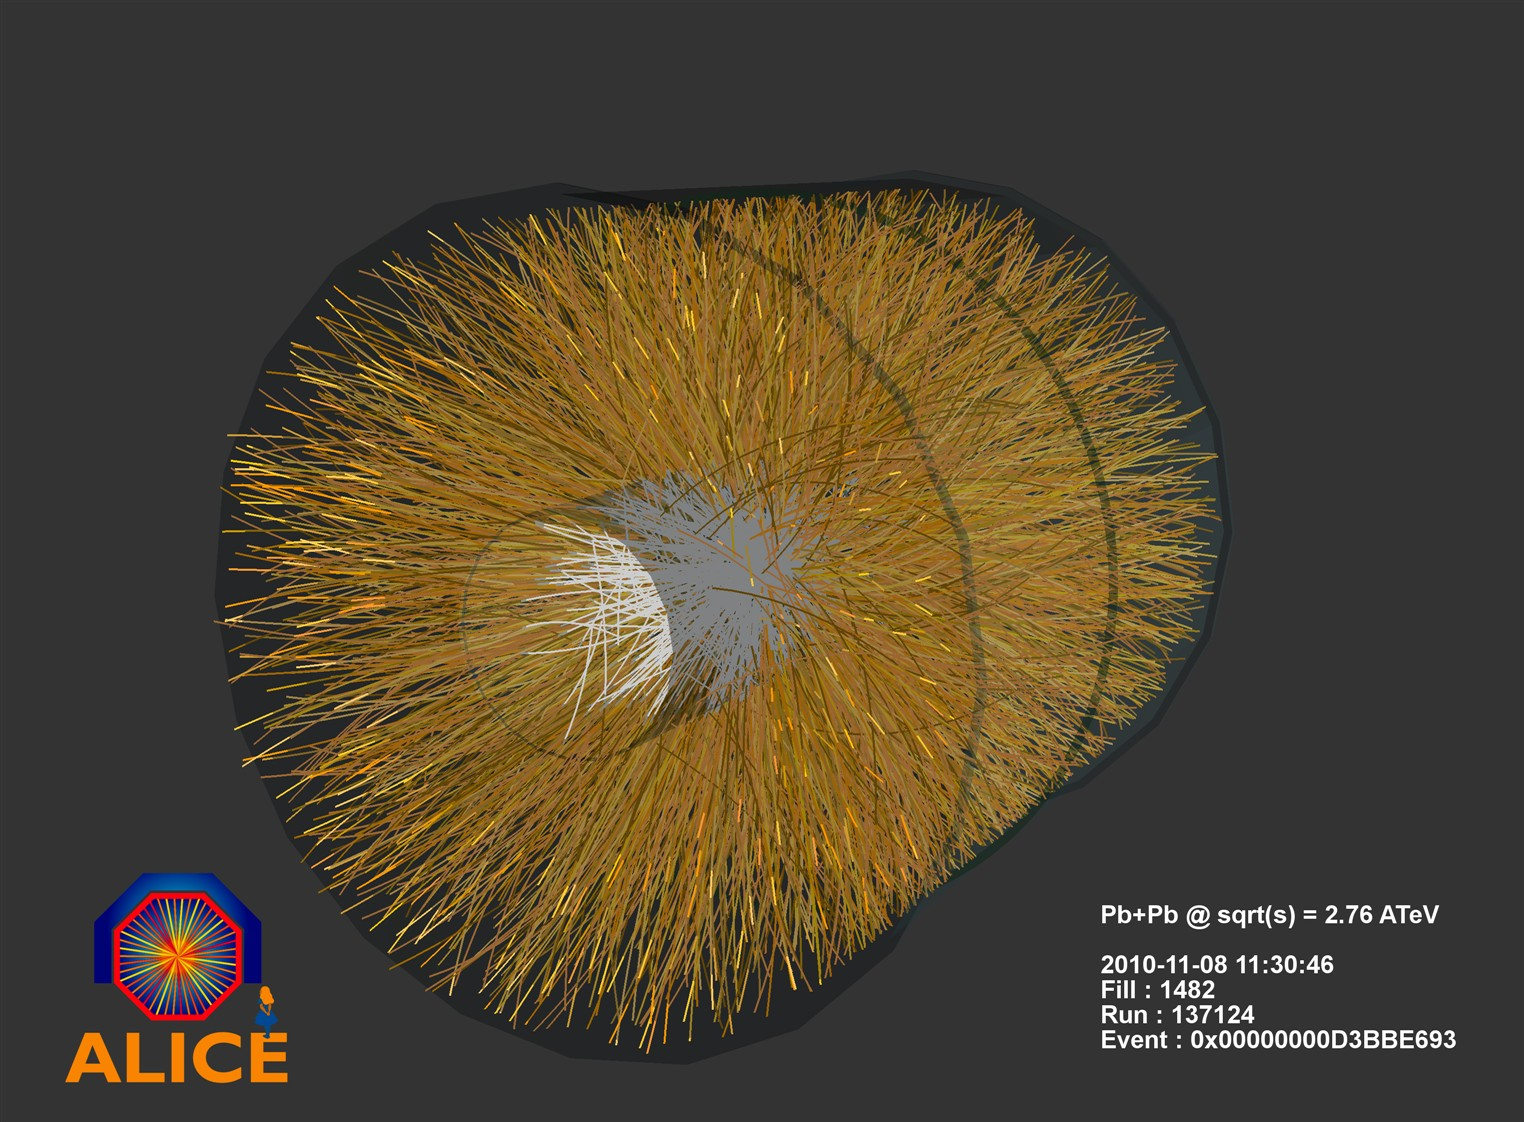
\includegraphics[width=.7\textwidth]{Pictures/alice.jpg}};
        \node at (1,-1) (star) {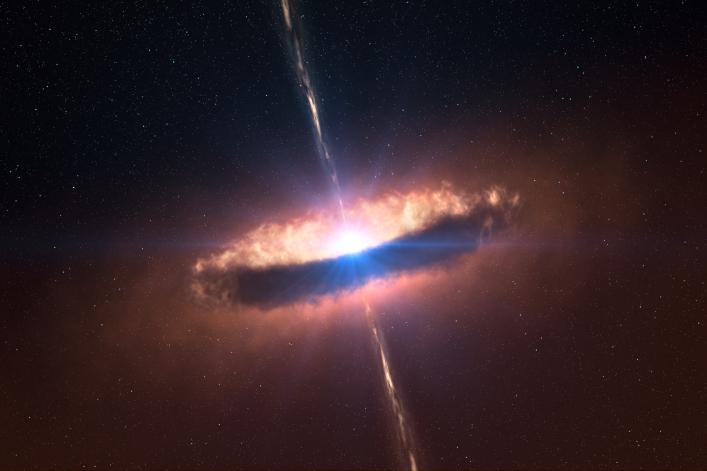
\includegraphics[width=.7\textwidth]{Pictures/massive_star.jpg}};
        \node at (star.south){\tiny Picture taken from \url{nasa.gov}};
      \end{tikzpicture}%
    }
    \only<3>{%
      \begin{tikzpicture}
        \node at (0,0) (alice) {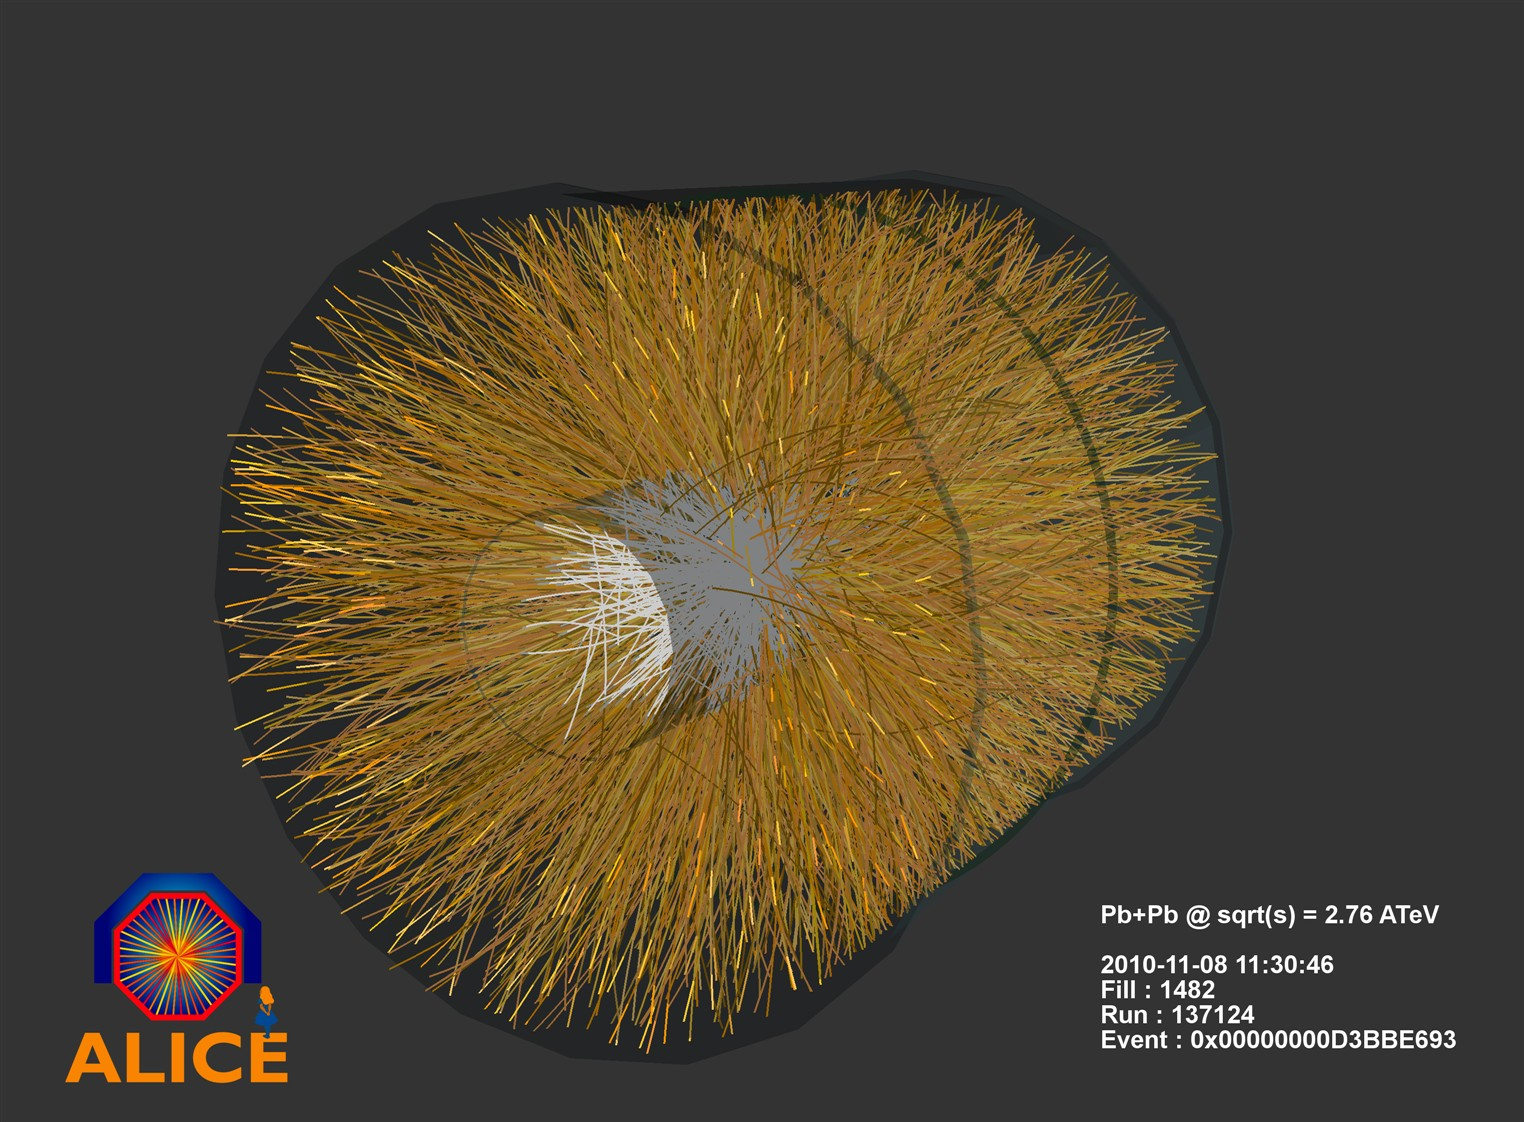
\includegraphics[width=.7\textwidth]{Pictures/alice.jpg}};
        \node at (1,-1) (star) {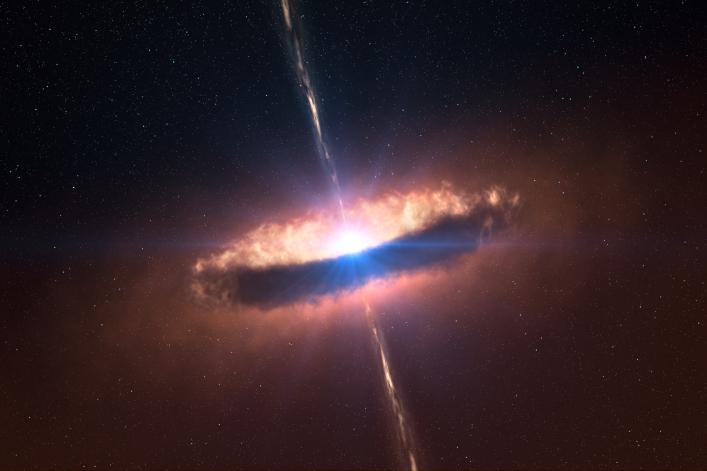
\includegraphics[width=.7\textwidth]{Pictures/massive_star.jpg}};
        \node at (-0.5,-1.5) (phase) {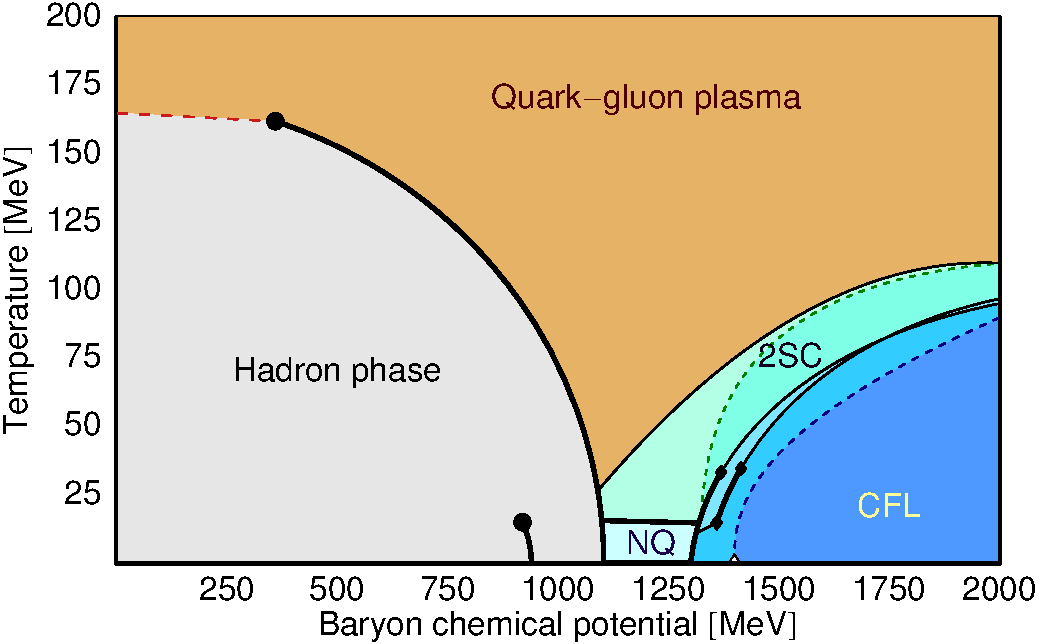
\includegraphics[width=0.7\textwidth]{Pictures/qcd_phase.pdf}};
        \node at (phase.south){\tiny \emph{Phys.Rev.}D72,n.3,p.1 (2005)};
      \end{tikzpicture}%
    }
  \end{columns}
\end{frame}

\footnotesize

\begin{frame}
  \frametitle{The Linear Sigma Model}
  \begin{block}{}
    \begin{equation*}
      \mathcal{L}_{\text{LSM}} = \frac{1}{2}\text{tr}\big[\partial_{\mu}\Phi^{\dagger}\partial^{\mu}\Phi\big] + U(\Phi)
    \end{equation*}
    \begin{equation*}
      U(\Phi) = \frac{1}{2}m^2\text{tr}\big[\Phi^{\dagger}\Phi\big] + \frac{\lambda_1}{4!}\Big(\text{tr}\big[\Phi^{\dagger}\Phi\big]\Big)^2 + 
      \text{tr}\big[h(\Phi^{\dagger} + \Phi)\big]  + \dots
    \end{equation*}
  \end{block}

  %\only<1>

  \only<2>{
    \begin{block}{$N_F = 2$}
      $\Phi = \displaystyle\frac{1}{\sqrt{2}} \begin{pmatrix} \sigma & 0 \\ 0 & \sigma \end{pmatrix} 
      + i\displaystyle\frac{1}{\sqrt{2}} \begin{pmatrix} \pi_0 & \pi_- \\ \pi_+ & \mathllap{-}\pi_0 \end{pmatrix}$
    \end{block}

    \begin{block}{$N_F = 3$}
      $\Phi = \displaystyle\frac{1}{\sqrt{2}} \begin{pmatrix}
        \frac{1}{\sqrt{2}} \sigma_{ud} + \frac{1}{\sqrt{2}} \mathrlap{a_0} & a_0^- & K_0^{*-} \\
        a_0^+ & \mathllap{\frac{1}{\sqrt{2}}} \sigma_{ud} - \frac{1}{\sqrt{2}} \mathrlap{a_0} & \bar{K}_0^* \\
        K_0^{*+} & K_0^* & \sigma_s
      \end{pmatrix} + \text{pseudo scalar mesons}$
    \end{block}
  }
\end{frame}

\begin{frame}
  \frametitle{\dots with quarks}

  \begin{block}{}
    \begin{equation*}
      \mathcal{L}_{\text{LSMq}} = \bar{\psi}\big(i\slashed{\partial} - g(\sigma + i\gamma^5\pi) \big)\psi +
      \mathcal{L}_{\text{LSM}}
    \end{equation*}
  \end{block}

  \begin{itemize}
    \item We have chiral symmetry of the quark Lagrangian when the fermionic fields are massless
    \item $\Rightarrow$ The degree of Chiral symmetry determined by $\langle \Phi \rangle$
    \item Which itself is determined by the thermodynamic potential 
  \[
    \Omega = -\frac{1}{V\beta} \, \text{log}\,\mathcal{Z}
  \]
  \end{itemize}
\end{frame}

\begin{frame}
  \frametitle{Perturbative methods}
  \framesubtitle{Mean Field Approximation}

  Simplest first approximation is at one-loop, where all mesonic quantum fluctuations are suppressed.

  \begin{block}{}
    \begin{equation*}
      \Omega[\Phi] = U(\Phi) + \Omega_{q\bar{q}}[\Phi]
    \end{equation*}
  \end{block}

  \begin{itemize}
    \item The physical free energy $\Omega$ is given at its minimum, $\Phi_0$, 
      \begin{equation*}
        \frac{\partial\Omega}{\partial\Phi} \Big|_{\Phi_0} = 0
      \end{equation*}
    \item where $\Omega_{q\bar{q}}$ is the free energy of $N_F$ massive free fermionic fields, with masses given by $\Phi_0$.
  \end{itemize}

\end{frame}

\begin{frame}
  \frametitle{Functional Renormalisation Group}
  \framesubtitle{Effective Average Action}

  \begin{alertblock}{\itshape Goal}
    Find the evolution of Gibb's free energy with respect to the renormalisation scale.
  \end{alertblock}
\end{frame}

\begin{frame}
  \frametitle{Functional Renormalisation Group}
  \framesubtitle{Effective Average Action}

  \begin{itemize}
    \item First regularise the action by using Pauli-Villars regularisation:
  \end{itemize}
  
  \begin{block}{}
    \begin{equation*}
      S[\phi] \rightarrow S[\phi] + \Delta_k[\phi] = S[\phi] + \frac{1}{2} \int \mathrm{d}^d p \, R_{k,i,j}(p) \phi_{p,i} \phi_{-p,j}
    \end{equation*}
  \end{block}

  \begin{itemize}
    \item Which in turns adds a renormalisation scale dependence to Gibb's free energy\footnote{\tiny being the Legendre transform of
      Helmholtz' free energy}
    \item Can in turn find a PDE for Gibb's free energy
  \end{itemize}

  \begin{block}{The Wetterich equation}
    \begin{equation*}
      \partial_k \Gamma_k = \frac{1}{2} \text{tr} \int_q \partial_k R_{k,i,j}(q) \Big( \frac{\delta^2 \Gamma_k}{\delta \phi_i(p) \delta \phi_j(p')} + 
      \delta(p + p') R_{k,i,j}(p)\Big)^{-1}_{q,-q}
    \end{equation*}
  \end{block}

  \begin{itemize}
    \item With an identical procedure for fermionic fields
  \end{itemize}
\end{frame}

\begin{frame}
  \frametitle{Functional Renormalisation Group}
  \framesubtitle{Local Area Approximation}

  \begin{itemize}
    \item Expand Gibb's free energy in powers of the $\partial$ operator, and truncate it
  \end{itemize}

  \begin{block}{$\mathcal{O}(\partial^2)$}
    \begin{equation*}
      \Gamma_k[\phi] = \int \mathrm{d}^d x \, \Big( \frac{1}{2}Z_k(\phi)(\nabla_4 \phi)^2 + U_k(\phi) \Big)
    \end{equation*}
  \end{block}

  \begin{itemize}
    \item Without the field renormalisation term $Z_k(\phi)$, the expansion is $\mathcal{O}(\partial^0)$, also known as the Local
      Area Approximation. In this expansion, the Wetterich eq. is:
  \end{itemize}

  \begin{block}{}
    \begin{equation*}
      \partial_k U_k = \frac{1}{2} \int_q \, \partial_k R_k(q) \bigg[ q^2 + \frac{\partial^2 U_k}{\partial\phi^2} +
      R_k(q)\bigg]^{-1}
    \end{equation*}
  \end{block}
\end{frame}

\begin{frame}
  \frametitle{Results}
  \framesubtitle{MF - Chiral phase transition}

  {\centering
    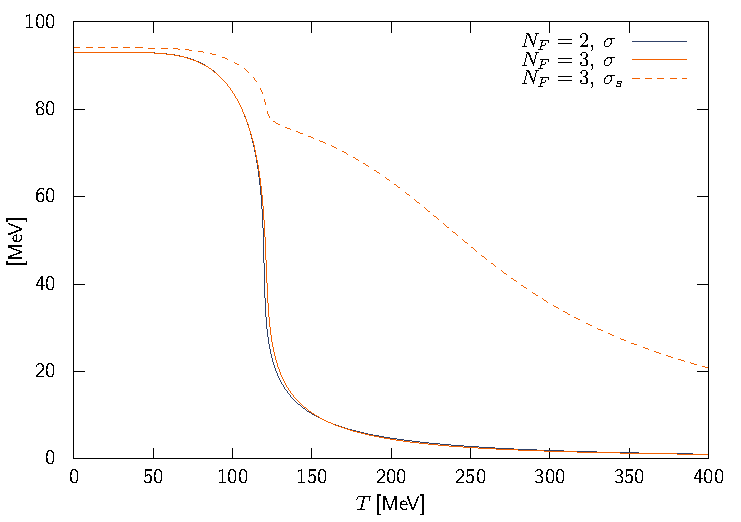
\includegraphics[width=0.9\textwidth]{Plots/mftrans.pdf}
   \par}
\end{frame}

\begin{frame}
  \frametitle{Results}
  \framesubtitle{MF - Chiral phase diagram}

  {\centering
    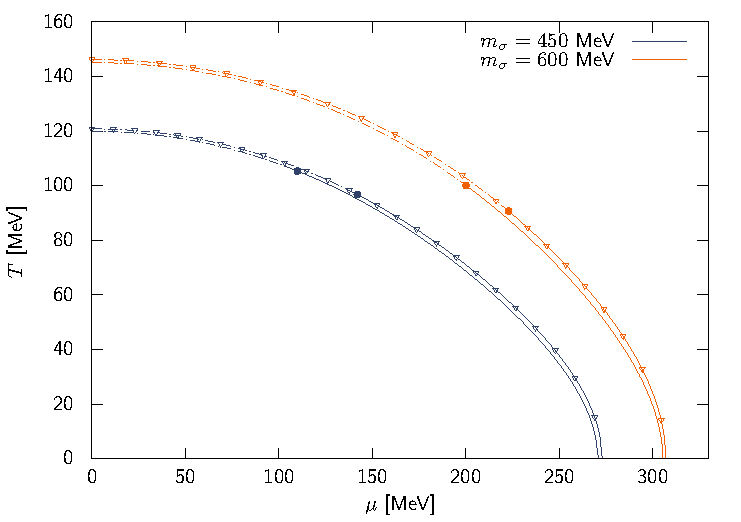
\includegraphics[width=0.9\textwidth]{Plots/2_3mixed.pdf}
   \par}
\end{frame}

\begin{frame}
  \frametitle{Results}
  \framesubtitle{RGE - Chiral phase transition}

  {\centering
    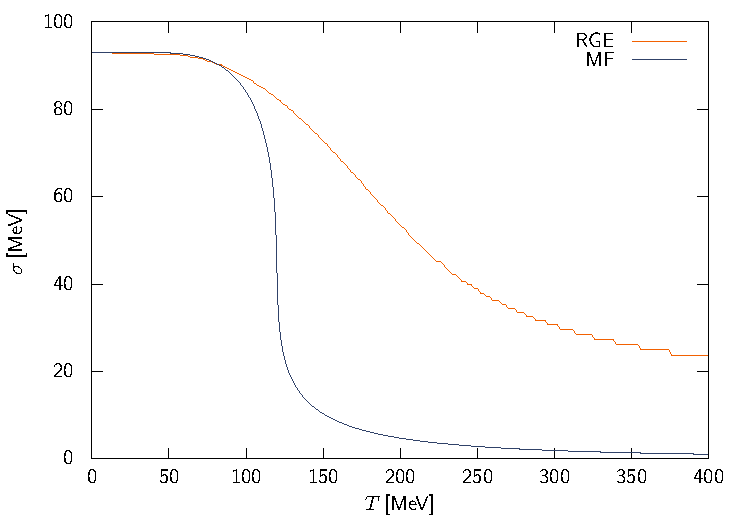
\includegraphics[width=0.9\textwidth]{Plots/rgetrans.pdf}
   \par}
\end{frame}

\begin{frame}
  \frametitle{Results}
  \framesubtitle{RGE - Chiral phase diagram}

  {\centering
    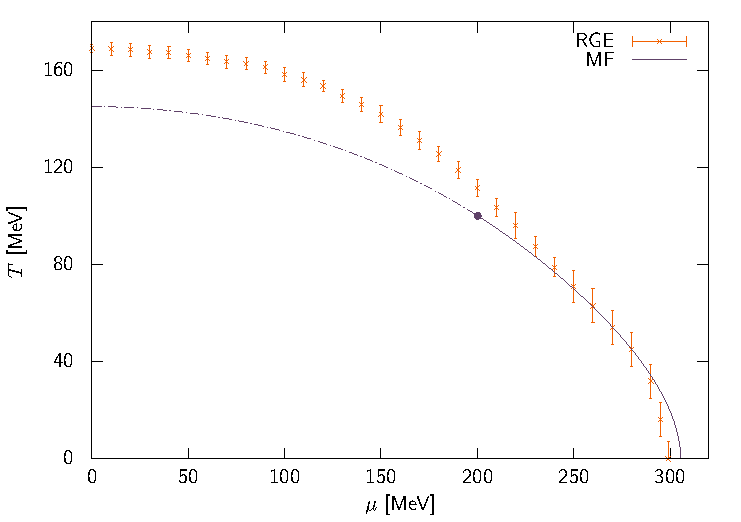
\includegraphics[width=0.9\textwidth]{Plots/rgediag.pdf}
   \par}
\end{frame}

\begin{frame}
  \frametitle{Summary}

  Got a short introduction to:
  \begin{itemize}
    \item The Linear Sigma Model with Quarks
    \item Symmetry considerations
    \item The perturbative Mean Field Approximation
    \item The nonpertbative Local Area Approximation
  \end{itemize}

\end{frame}

\end{document}


